\documentclass[a4paper, 12pt, twoside]{article}

\usepackage{grugraStyle}

\title{\Huge \textbf{
\textsf{Gruppen und Graphen}}}
\date{}

\setcounter{tocdepth}{2}

\makeindex

% --------------------
\begin{document}

\maketitle
\begin{center}
	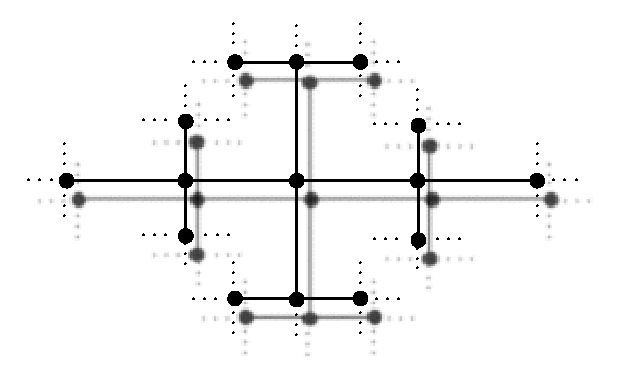
\includegraphics{titel}
\end{center}
\newpage
\tableofcontents
\newpage

\include{graphen}

\include{cayley}

\include{serre}

\appendix


%--------- Literatur

\newpage
\begin{thebibliography}{10}
\addcontentsline{toc}{section}{Literatur}

\bibitem{diestel} \textsc{R. Diestel}\\
\textsl{Graphentheorie}\\
Springer 2006\\
\textsf{http://www.math.uni-hamburg.de/home/diestel/books/graphentheorie/}

\bibitem{globke} \textsc{M. Grassl, W. Globke}\\
\textsl{Algorithmen für Gruppen und Codes}\\
\textsf{http://www.stud.uni-karlsruhe.de/$\sim$uy7t/zeugs/}

\bibitem{hatcher} \textsc{A. Hatcher}\\
\textsl{Algebraic Topology}\\
Cambridge University Press 2001\\
\textsf{http://www.math.cornell.edu/$\sim$hatcher/AT/ATpage.html}

\bibitem{lang} \textsc{S. Lang}\\
\textsl{Algebra}\\
Springer 2002

\bibitem{serre} \textsc{J.P. Serre}\\
\textsl{Trees}\\
Springer 1980



\end{thebibliography}

\newpage
\addcontentsline{toc}{section}{Index}
\small
\printindex


\end{document}
